% !TEX root = pa_doc.tex
\begin{markdown}

# Implementation

## Architecture

ZHAWo consists of a frontend React \cite{React} web application and a backend server based on the Node.js \cite{Node} package Express \cite{Express}. The frontend communicates with the backend through a REST API. The backend server itself - apart from providing the API for the frontend - communicates with the CampusInfo REST API provided by the ZHAW and the RSS feed of the vszhaw homepage. The CampusInfo API provides timetable and menu plan information.

\bigskip

\begin{figure}[H]
  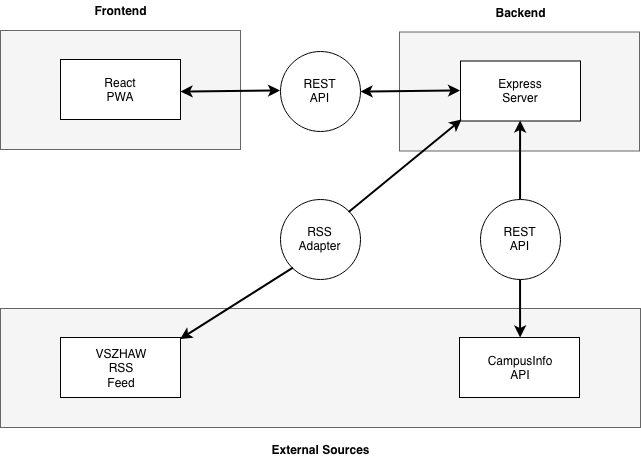
\includegraphics[width=14cm, center]{../diagrams/applicationArchitecture.png}
  \caption{\textsf{Application Architecture Diagram}}
\end{figure}

\bigskip

## Backend

The backend consists of the following modules:

\begin{itemize}
  \item \textbf{Express server application}: Handles HTTP requests from frontend and redirection to persistance layer or third-party adapters.
  \item \textbf{Persistence layer}: Handles caching of more resource intensive requests such as room search. Implemented with basic file system using JSON file in the prototype. Can be extended by database if functionality requires.
  \item \textbf{REST API adapter}: Handles HTTP fetch requests to the CampusInfo API.
  \item \textbf{RSS feed adapter}: Handles fetching of RSS feed from vszhaw.
\end{itemize}

### Express server application

For the backend server application, we have chosen to use the framework Express \cite{Express} based on the Node.js \cite{Node} technology. The server provides access to the React web application and also offers a REST API. The primary responsibility of the server is to redirect user request from the frontend to either persistence layer or the different API adapters and then serve the data. We have chosen to implement the backend with a JavaScript based framework so there is no technology difference between front- and backend. In the context of agile development in a small team, this allows for a fast implementation of features. A new feature often requires changes to both front- and backend, and by removing the need to switch context between different programming languages, we were able to maintain a good velocity throughout our sprints.

### Persistence layer

In the scope of developing this prototype, there was no need to implement a full database for data persistence. The data for more resource intensive requests such as the search for free rooms is currently stored in JSON format directly in the servers file system. Less intensive requests such as timetables are delivered from CampusInfo in a format that only needs minimal modifications and are directly sent to the frontend without persistence.

However, should the need for a database later arise through new functionality, integration into the Express server application is already prepared.

### REST API adapter

Most of the application data for ZHAWo is provided by the CampusInfo API. Since this is a third-party API provided by the ZHAW, we decided to implement an additional layer between our backend application core and the API. This insures that we are flexible to changes to CampusInfo.

### RSS feed adapter

Similarly to the CampusInfo API adapter, the RSS feed adapter provides an additional layer between our application and the RSS feed of the vszhaw. This ensures that should the data received by this third-party feed change, the changes needed to our application will be isolated to the adapter.

\newpage

## Frontend

The frontend is made up of three main parts:

\begin{itemize}
  \item \textbf{React web application}: Handles presentation of data and user interaction.
  \item \textbf{REST API adapter}: Handles HTTP fetch requests to the backend.
  \item \textbf{Service worker}: Handles PWA functionality such as caching of data for offline use and installation to desktop or phone homescreen.
\end{itemize}

### React web application

For the presentation of the web application to the user, we used the React framework \cite{React}. React was originaly developed by Facebook and is one of the most popular UI libraries in web development. It is based on reusable components built with JSX, a syntax extension to JavaScript. We decided to use React because of its component based modularity, which works well with an agile development approach where multiple features need to be implemented simultaniously with little interference.

To handle the application data we chose to use the Flux design pattern \cite{Flux}. Using the Flux pattern ensures a unidirectional data flow from view components through actions into a single dispatcher into data stores, where the application data such as timetables and menu plans is handled. In Flux, the dispatcher is a singleton that directs the flow of data to ensure that updates do not cascade, which would lead to unpredictable behaviour. When a user interacts with a React view, the view sends an action through the dispatcher, which notifies the stores that hold the application’s data. When the stores change state, the view gets notified and changes accordingly \cite{Flux}.

\bigskip

\begin{figure}[H]
  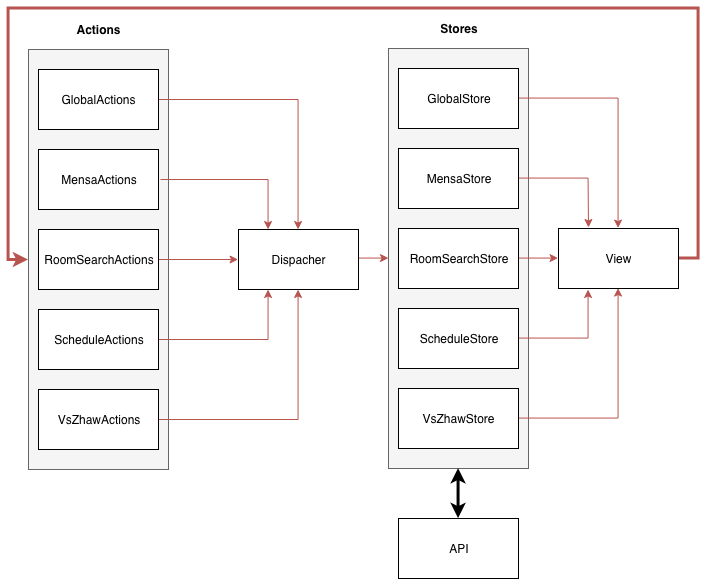
\includegraphics[width=11.3cm, center]{../diagrams/flux.png}
  \caption{\textsf{Flux Pattern Diagram}}
\end{figure}

\bigskip

### REST API adapter

The data such as timetables, menu plans or lists of free rooms are provided by the backend REST API. To ensure modularity between front- and backend, we implemented an adapter module that handles all data requests to the backend. This practice allows easier adaptations to changes in API, as only the adapter would have to be changed, while the other parts such as the React application and service worker do not need to change.

The modularity this design choice provides - similarly to the modularity of React - goes well with the agile principle of fast prototyping of new ideas and features.

### Service worker

The data for the frontend is provided by the backend REST API. All data received from HTTP fetch requests is cached using a service worker \cite{ServiceWorker}. By caching the application data, we ensure that the user can still access all the information that was already loaded once. It also improves the loading speed of ZHAWo, since resources that have been cached are first served from cache, before the data is requested by the backend. After the fetch request has completed the cache is updated. With regard to ,for example, a students schedule information, this practice makes a lot of sense since the actual data does not change often during the course of a semester.

In addition to offline caching, the service worker also allows users to install ZHAWo as a Progressive Web App (PWA) \cite{WhatIsPWA} to either their desktop or their phones homescreen.

These two features enables us to offer the experience of a native application while we avoid having to maintain separate code bases for each platform.

Google provides the automated tool Lighthouse \cite{Lighthouse} to audit and rate PWAs. Lighthouse various PWA aspects, including if the application still responds without network connection. ZHAWo achieved a score of 92 out of 100. A detailed report can be found on the Github Repository \cite{OurGithub}.

## Test Coverage

For testing we used the framework Jest \cite{Jest} for both front- and backend. To test functionality and output of React components, we used the GUI testing framework \cite{Enzyme} in addition to Jest.

For the express server application, we achieved a test coverage of 62\%. For the frontend React application 53\% of the code was covered, resulting in an overall project test coverage of about 55\% \cite{OurCoverage}. The coverage is lower than we had planned and is something we aim to improve when going from application prototype to production ready application. This can be in part attributed to the prototypical implementation of the primary functions menu plan, room search and student events. Another aspect is that the current JavaScript framework environment is very dynamic and fast paced, which on one hand offers many advantages, on the other hand, best testing practices have not been established. For example, it was challenging to isolate and test the different components of the Flux architecture in the frontend. Therefore, we decided to put a lot of focus on establishing better testing practices in the next stage of this project.

\newpage

## User Interface

The user interfaced was designed to provide students with the familiar look and feel of a native mobile application. We chose a minimalistic design approach. The focus was on displaying relevant information without any distracting noise or clutter.

The mockups were made so that both of us could work independently and no design decisions had to be made on the go. It was important to us to have a consistent design throughout the application.

\begin{figure}[H]
  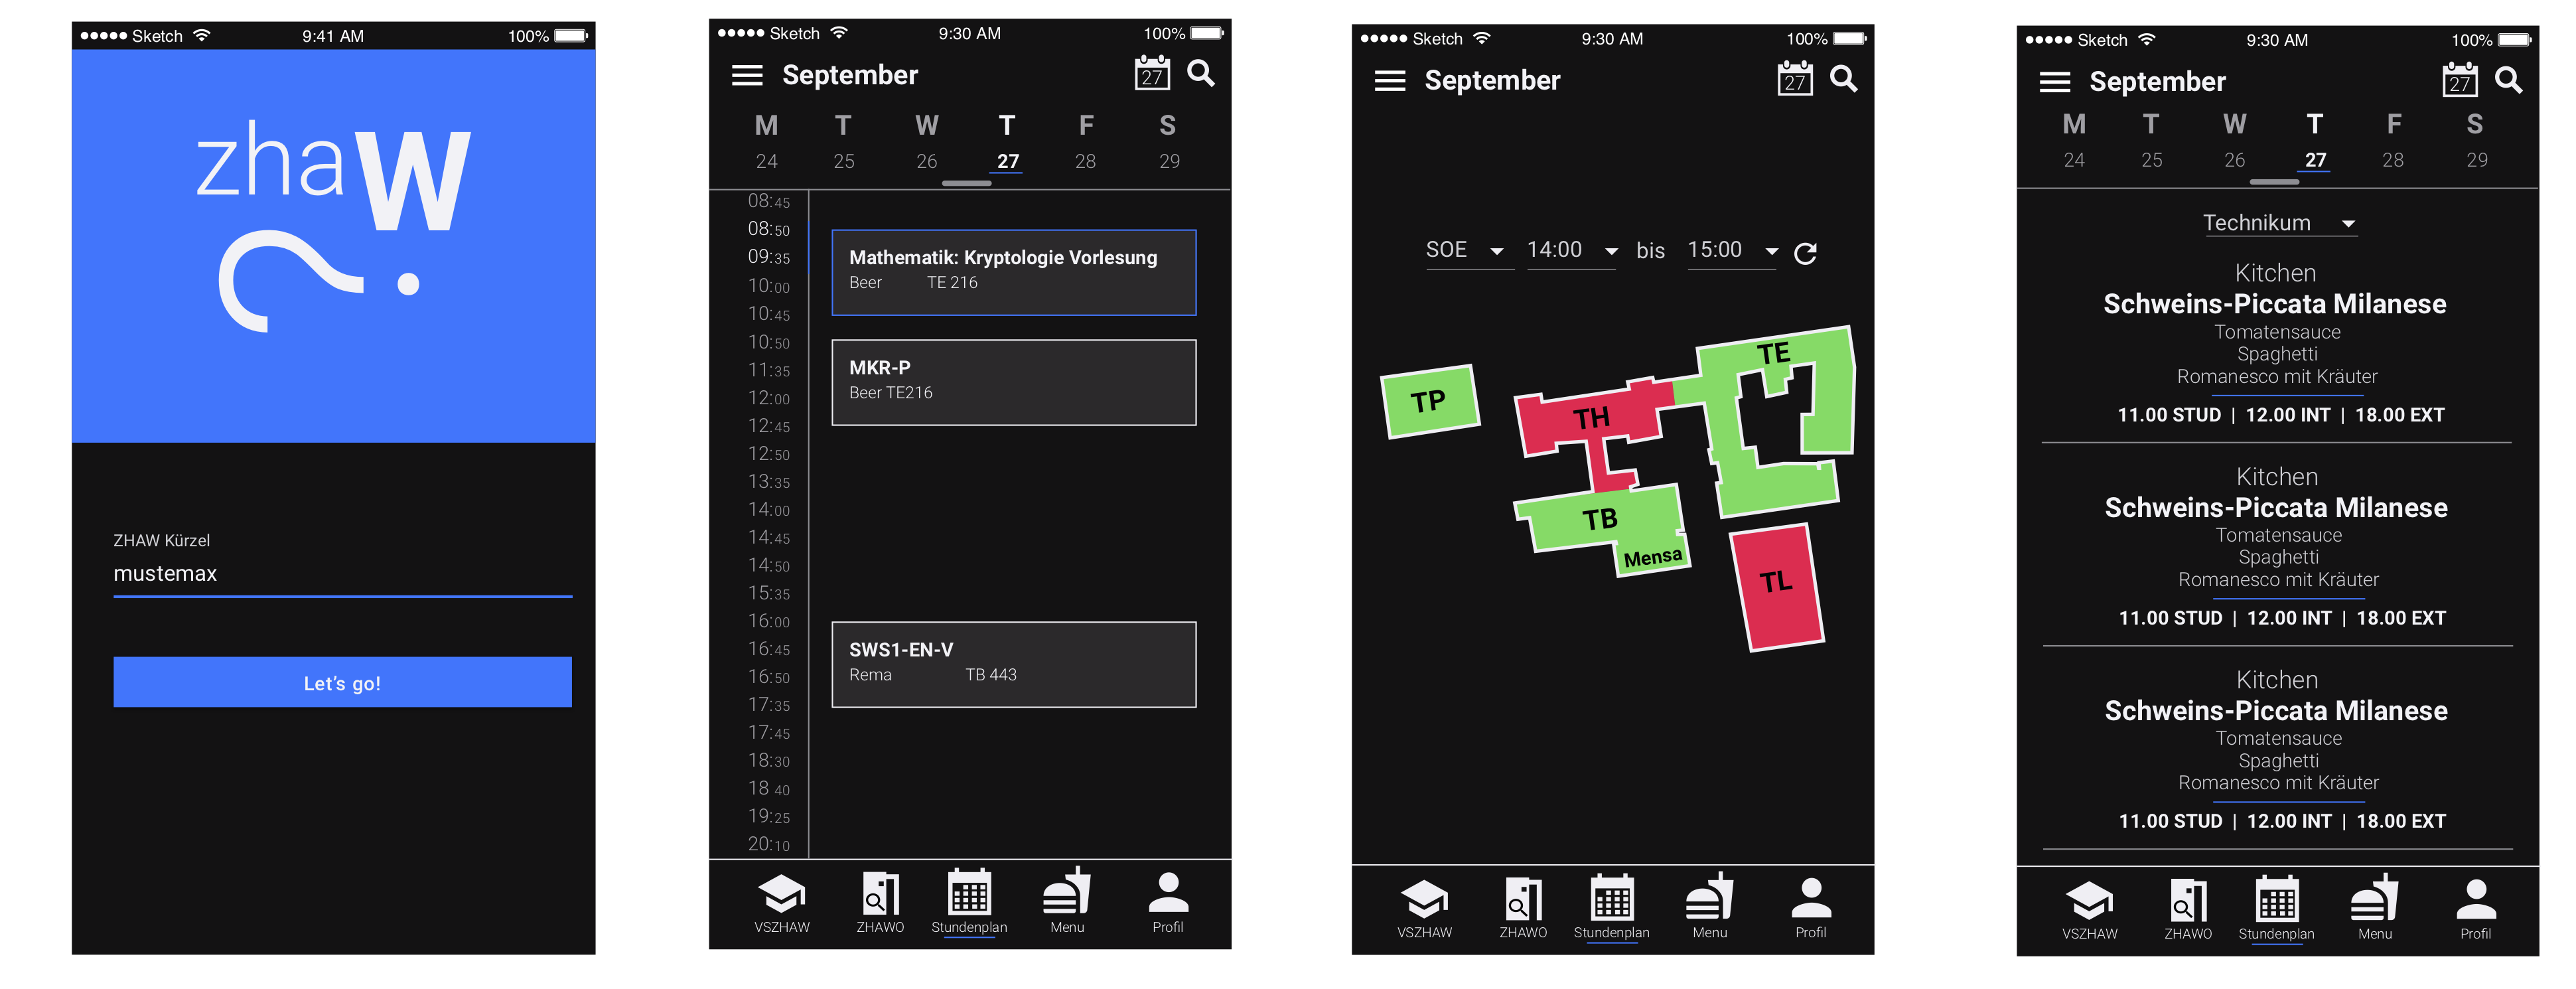
\includegraphics[width=16cm, center]{../Mockups/Mobile_Mockups.png}
  \caption{\textsf{Mobile Mockups}}
\end{figure}

The initial mockups were made with a dark theme. Our first user feedback on the design was very positive, but we learned that most users preferred a light theme over our dark theme. We decided to changed the default theme, whilst still leaving the option for users to change to the dark theme if preferred.

\begin{figure}[H]
  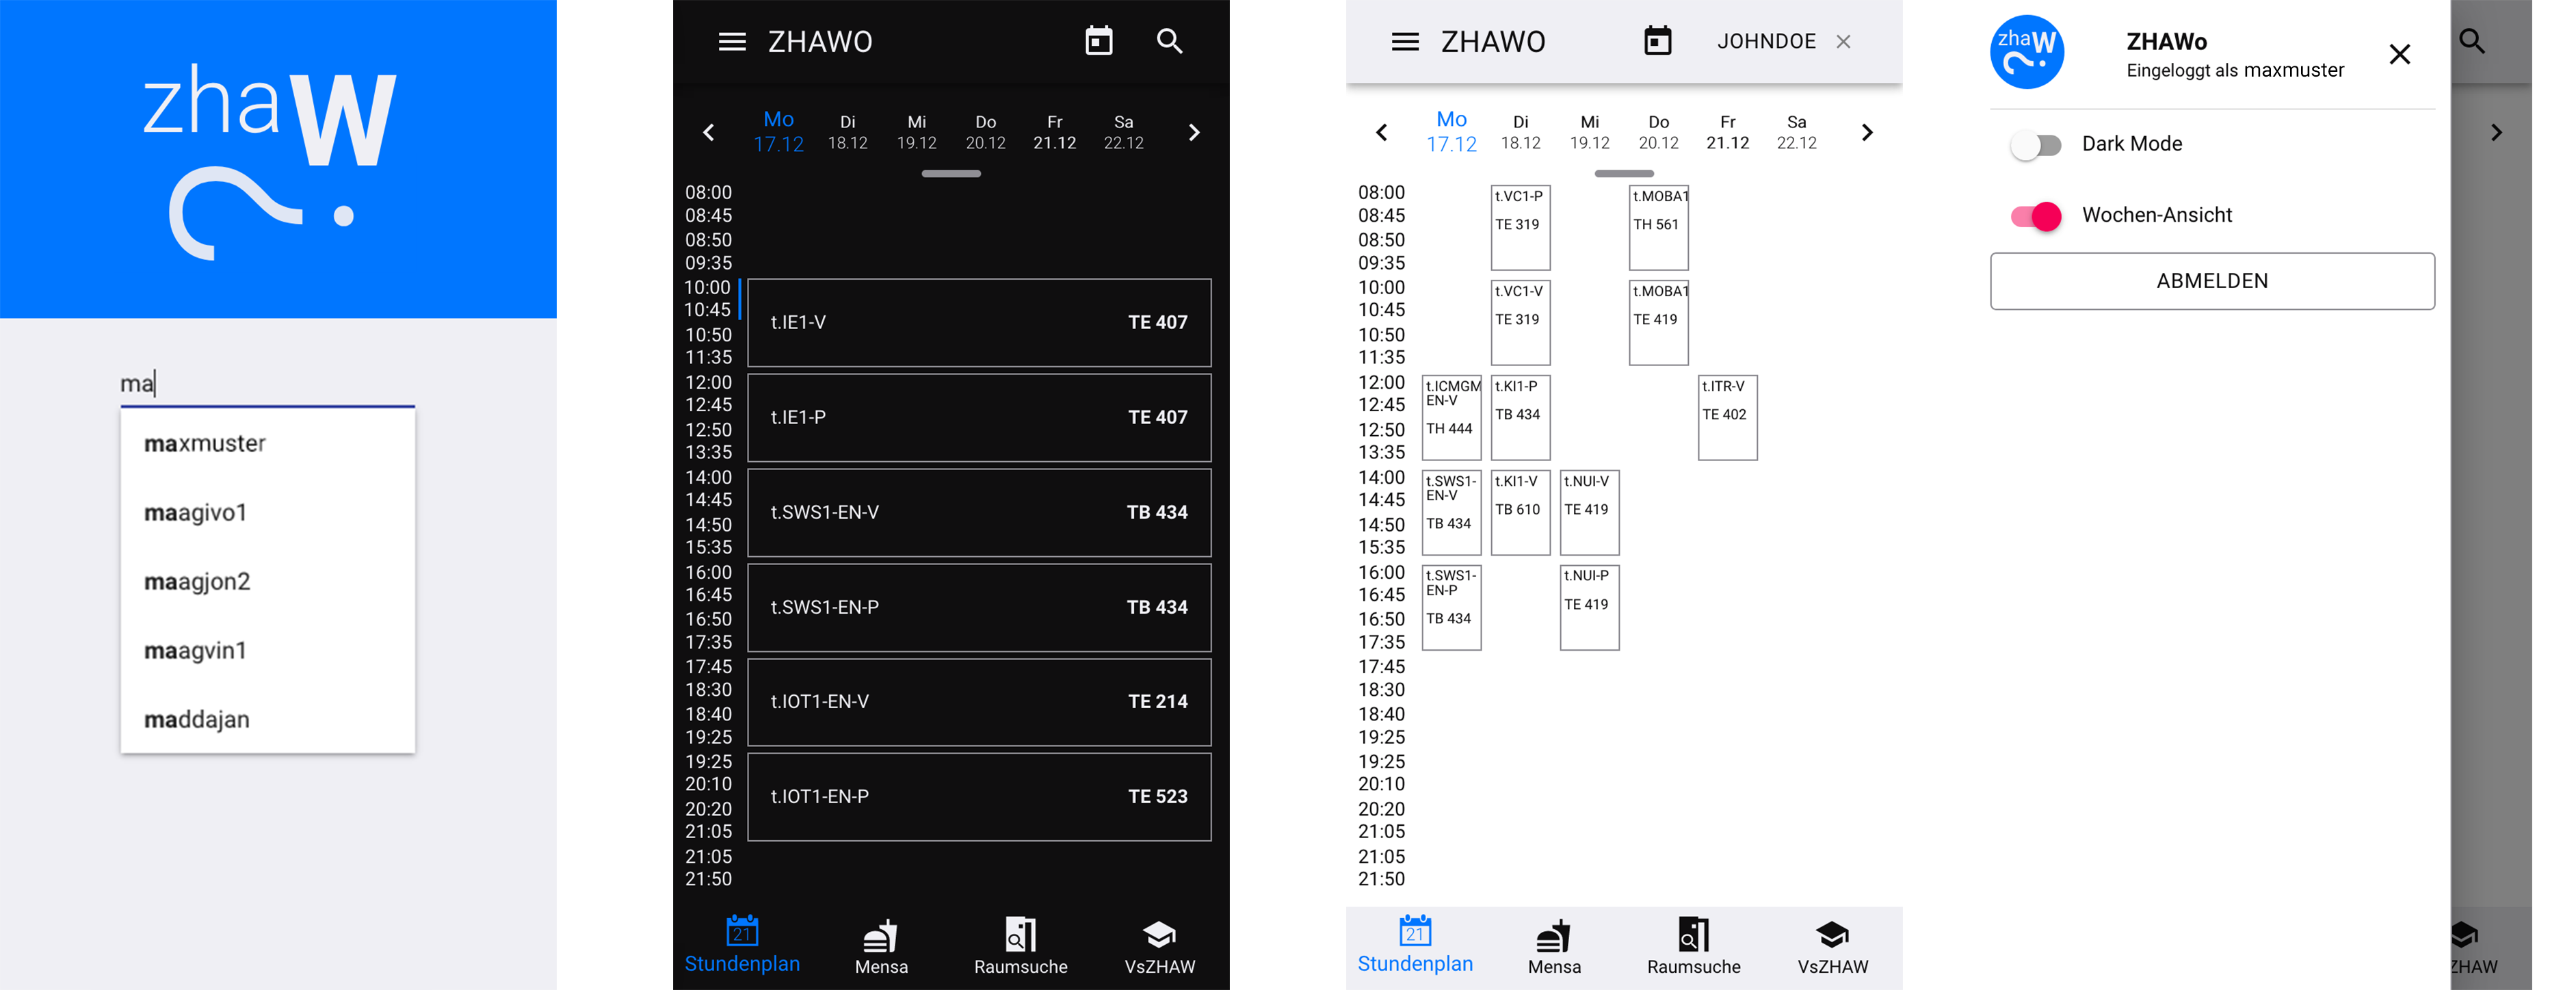
\includegraphics[width=16.5cm, center]{../Mockups/screenshots.png}
  \caption{\textsf{Mobile Screenshots}}
\end{figure}

\end{markdown}
